\section*{Anexo A -- Tabela de Indicadores de Qualidade do Serviço}
\label{anexo-tabela-indicadores}
\begin{table}[H]
\centering
\caption{Indicadores do serviço adequado. }
\resizebox{\textwidth}{!}{%
\begin{tabular}{ccccc}
\textbf{\begin{tabular}[c]{@{}c@{}}PARÂMETRO\\ DO SERVIÇO\\ ADEQUADO\end{tabular}} & \textbf{\begin{tabular}[c]{@{}c@{}}DEFINIÇÃO DO\\ PARÂMETRO\end{tabular}} & \textbf{\begin{tabular}[c]{@{}c@{}}INDICADOR\\ EQUIVALENTE\end{tabular}} & \textbf{SIGLA} & \textbf{\begin{tabular}[c]{@{}c@{}}DEFINIÇÃO\\ ADOTADA NO\\ INDICADOR\end{tabular}} \\ \hline
Regularidade & \begin{tabular}[c]{@{}c@{}}Prestação do serviço\\ conforme contrato, sem\\ interrupções\end{tabular} & Pontualidade & $P_N$ & \begin{tabular}[c]{@{}c@{}}Oferta do serviço de\\ forma contínua e\\ conforme planejado\end{tabular} \\ \hline
Continuidade & \begin{tabular}[c]{@{}c@{}}Manutenção da oferta\\ em caráter permanente\end{tabular} & Tempo & $T_E$ & \begin{tabular}[c]{@{}c@{}}Tempo de realização\\ da viagem, incluindo\\ transbordos\end{tabular} \\ \hline
Eficiência & \begin{tabular}[c]{@{}c@{}}Atendimento ao usuário\\ com o melhor uso dos\\ recursos\end{tabular} & Lotação & $L_O$ & \begin{tabular}[c]{@{}c@{}}Oferta de lugares e\\ conforto das viagens\end{tabular} \\ \hline
Segurança & \begin{tabular}[c]{@{}c@{}}Confiança oferecida ao\\ usuário na prestação do\\ serviço\end{tabular} & Segurança & $S_G$ & \begin{tabular}[c]{@{}c@{}}Serviço seguro, sem\\ incidência de\\ acidentes e assaltos\end{tabular} \\ \hline
Atualidade & \begin{tabular}[c]{@{}c@{}}Modernidade de\\ técnicas, equipamentos\\ e instalações\end{tabular} & Informações & $I_F$ & \begin{tabular}[c]{@{}c@{}}Uso de técnicas para\\ fornecer informação\\ ao usuário, sem\\ necessidade de\\ solicitação\end{tabular} \\ \hline
Generalidade & \begin{tabular}[c]{@{}c@{}}Serviço com\\ atendimento a todos os\\ usuários, sem distinções\end{tabular} & Veículos & $V_E$ & \begin{tabular}[c]{@{}c@{}}Acesso de pessoas\\ com necessidades\\ especiais e\\ conservação dos\\ veículos\end{tabular} \\ \hline
Cortesia & \begin{tabular}[c]{@{}c@{}}Serviço prestado com\\ urbanidade ao usuário\end{tabular} & Tripulação & $T_R$ & \begin{tabular}[c]{@{}c@{}}Comportamento dos\\ operadores e sua\\ relação com usuários\end{tabular} \\ \hline
\begin{tabular}[c]{@{}c@{}}Modicidade das\\ tarifas\end{tabular} & \begin{tabular}[c]{@{}c@{}}Tarifas compatíveis\\ com a renda do usuário\end{tabular} & Tarifa & $T_A$ & \begin{tabular}[c]{@{}c@{}}Representatividade\\ da tarifa na renda do\\ usuário\end{tabular} \\ \hline
\end{tabular}%
}
Fonte: \cite[p. 43]{MARTINS}
\label{cotran-table}
\end{table}

\chapter*{Anexo B -- Métodos Exatos Utilizados no VRP}
\label{anexo-metodos-exatos}
\subsection*{Branch-and-bound}
Esta estratégia consiste em solucionar problemas de otimização com restrições de variáveis inteiras. A partir de um problema inicial, é criada uma série de ramificações (\emph{Branch}) das restrições (\emph{Bound}) que existem no problema, de modo que as restrições não permitam uma solução parcial do problema. Esta estratégia construi uma árvore de decisão com base em limites superiores e inferiores, impedindo que algumas soluções ruins sejam exploradas. Este método pode ser utilizado com outros métodos de programação linear, como por exemplo, o SIMPLEX \cite{LAPORTE1992345}. O \emph{Branch-and-Bound} elimina ramificações de restrições caso se encontre uma das condições:

\begin{enumerate}
    \item O problema restrito é impossível.
    \item A solução ótima do ramo é inteira.
    \item A solução encontrada no ramo é pior do que a melhor solução atual.
\end{enumerate}

\subsection*{Branch-and-cut}
Esta estratégia é uma melhoria do algoritmo \emph{Branch-and-bound}. Nela, ocorre a resolução dos problemas relaxados (sem restrições de integralidade) do \emph{Branch-and-bound}, utilizando um plano de cortes. O algoritmo percorre em cada nó da árvore, executando o plano de cortes e checando se naquele nó, a solução ótima do subproblema obedece às restrições de integralidade ou se o limitante inferior é maior que a solução já conhecida e caso uma dessas situações ocorra, o nó é descartado. Caso não seja encontrada uma inequação válida para o problema de separação, aplica-se a ramificação.

\subsection*{Branch-and-price}
Em casos de problemas de otimização com variáveis integrais, onde se considera todas as variáveis do problema simultaneamente, torna-se inviável a utilização das estratégias anteriores. Visto esse tipo de problema, foi criada uma técnica chamada de Geração de Colunas, com intuito de resolver esse tipo de problema. A técnica visa selecionar variáveis com o maior potencial para otimizar o problema. A estratégia \emph{Branch-and-price} é uma versão da estratégia \emph{Branch-and-bound}, que utiliza a Geração de Colunas  em cada nó da árvore de decisão.

\chapter*{Anexo C -- Métodos Heurísticos Utilizados no VRP}
\label{anexo-metodos-heuristicos}
\subsection*{Clarke e Wright}
Esta foi uma estratégia extremamente importante para o desenvolvimento dos algoritmos voltados ao VRP pois serviu como base para a construção de outros algoritmos sofisticados de roteamento de rotas e veículos \cite{milton-nascimento}. O algoritmo cria grafos contendo os clientes e possíveis rotas, já o depósito é lido a partir de alguma estrutura de armazenamento, então, são calculadas \emph{n-1} rotas de um cliente ao depósito onde n é o número de nós do grafo. A partir destes pares de nós, é calculado  o custo da rota a partir da fórmula \cite[p. 32]{maxwell}: 

\[ s_{ij} = c_{i0} + c_{0j} - c_{ij} \]

$s_{ij}$ representa a economia com relação aos nós \emph{i} e \emph{j}, e $c_{ij}$ representa o custo de se ir do nó \emph{i} ao nó \emph{j}. As economias são colocadas, em ordem decrescente, em uma tabela após o cálculo. 

O algoritmo de \emph{Clark e Wright} é executado em tempo polinomial, pois, a complexidade é da ordem $\mathcal{O}(n^2)$. Há, no entanto, uma desvantagem de se usar a estratégia de \emph{Clark e Wright}, pois o algoritmo descartará todos os nós que não se encontram nos extremos das rotas, ou seja, os nós internos não entram na tabela de economia.
\subsection*{Mole e Jameson}

A estratégia de \emph{Mole e Jameson} é uma melhoria do algoritmo de \emph{Clark e Wright}, ele tem como um ponto forte, considerar os nós internos que são descartados no teste de economia do algoritmo de \emph{Clark e Wright}. O algoritmo começa carregando o grafo a partir de uma matriz de adjacências e de uma lista de nós livres (nós que não pertencem à nenhuma rota). Posteriormente, é construído um grafo que não contém o nó do depósito a partir da matriz de adjacências e da lista de nós livres. A partir de algum critério pré-definido, um par de nós é escolhido para ser a rota inicial. Após definida a rota inicial, um laço começará a inserir os nós na rota, seguindo dois critérios: O de \textbf{Proximidade} e o de \textbf{Economia}.
Para realizar o cálculo da \textbf{Proximidade} dos nós é utilizada a seguinte fórmula \cite[p. 33]{maxwell}:

\[\alpha(i, k, j) = c_{ik} + c_{kj} - \lambda c_{ij} \]

Onde $c_{ik}$ representa o custo entre os nós \emph{i} e \emph{k}, $c_{kj}$  representa o custo entre os nós \emph{l} e \emph{j}. Se nenhuma violação for quebrada, o nó com menor distância será inserido na rota. O cálculo da economia é aquele que apontará qual o melhor lugar para o nó ser inserido, este cálculo é dado por:

\[\beta(i, k, j) = \mu 0k - \alpha(i, k, j) \]


Onde \(\mu 0k\) representa a distância entre o depósito e o nó $l$. O local selecionado representa o que tem mais economia.

\chapter*{Anexo D -- Métodos Meta-Heurísticos Utilizados no VRP}
\label{anexo-metodos-metaheuristicos}
\subsection*{Busca Tabu}

A etimologia da palavra \emph{tabu} tem origem do \emph{Tongan}, idioma falado em Tonga, na Polinésia e indica algo proibido por ser sagrado e que não pode ser tocado ou mencionado. O algoritmo da busca tabu é assim nomeado por ser composto de estratégias que permitem \emph{proibir} determinadas ações durante a varredura de vizinhanças e a escolha de soluções.

A busca tabu foi introduzida na literatura por Fred Glover em 1986 \cite{GLOVER1986533} e posteriormente aperfeiçoada em outros trabalhos acadêmicos. É um método que permite tanto uma abordagem probabilística \cite{crainic1993dynamic} quanto determinística \cite{ongsakul2004unit}. Ao contrário de muitos métodos meta-heurísticos, a busca tabu não possui analogia com fenômenos naturais. Os princípios de uma busca tabu segundo Golbarg \emph{et al.} (2015) são:
\begin{enumerate}
    \item Uma busca eficiente não deve revisitar soluções;
    \item Manter registro de todas as soluções visitadas é computacionalmente dispendioso. É mais eficiente armazenar alterações na solução ou em variáveis;
    \item Memorizar alterações nas soluções não elimina a possibilidade de reexame de soluções, apenas diminui a chance dessa possibilidade.
\end{enumerate}

Um dos princípios da busca tabu é aproveitar-se de um esquema de gestão de memória auxiliar de curto, médio e longo prazo para evitar examinar mais de uma vez uma mesma configuração em uma varredura em busca de uma solução. Este conjunto de proibições -- usualmente denominado \emph{condições tabu} -- é registrado em memória dinâmica, permitindo que seja alterado de acordo com o progresso da busca, visto que podem ocorrer evidências de que uma configuração de solução não está sendo considerada e estas proibições precisam ser desativadas. Além de evitar repetições, uma otimização das configurações da busca permite aumentar a chance da busca escapar da atração de mínimos locais. 

Fundamentalmente, algoritmos de busca tabu são orientados à varredura de vizinhanças específicas (denominada \emph{intensificação}) com configuração de foco de busca variável (denominada \emph{diversificação}). Um algoritmo de busca tabu visa crucialmente minimizar a quantidade de configurações visitadas e fornecer condições de escape de mínimos locais. Portanto, para atingir este objetivo, uma busca tabu é composta por:

\begin{itemize}
    \item Memória de curto prazo para preservar o histórico imediato da busca;
    \item Estratégias de memória de médio e longo prazo com o objetivo de equilibrar o esforço computacional da \emph{intensificação} com o utilizado na \emph{diversificação};
    \item Regras que permitam ajustar gestão da memória, critérios de pertubação e de escolha da configuração.
\end{itemize}

A busca tabu armazena na memória algumas soluções e armazena as alterações posteriores nas próprias soluções. Estas modificações nas soluções são denominadas de \emph{pertubações}. Uma \emph{pertubação} é uma alteração no valor ou na composição das variáveis de uma solução. Goldbarg \emph{et al.} (2015) exemplificam alguns exemplos de possíveis movimentos em uma configuração:

\begin{itemize}
    \item Mudar as atribuições de uma variável binária de zero para um, ou vice-versa.
    \item Permutar os vértices em uma solução de rota.
    \item Introduzir ou retirar arcos em uma grafo solução.
    \item Alterar as atribuições realizadas sobre os vértices de um grafo solução.
\end{itemize}

A figura \ref{taboo-image} representa através de um fluxograma o passo a passo de um algoritmo de Busca Tabu. Os comentários identificam o propósito e o nome de cada passo. 


\begin{figure}[H]
  \centering
  \caption{Passo a passo com comentários de um algoritmo de Busca Tabu.}
 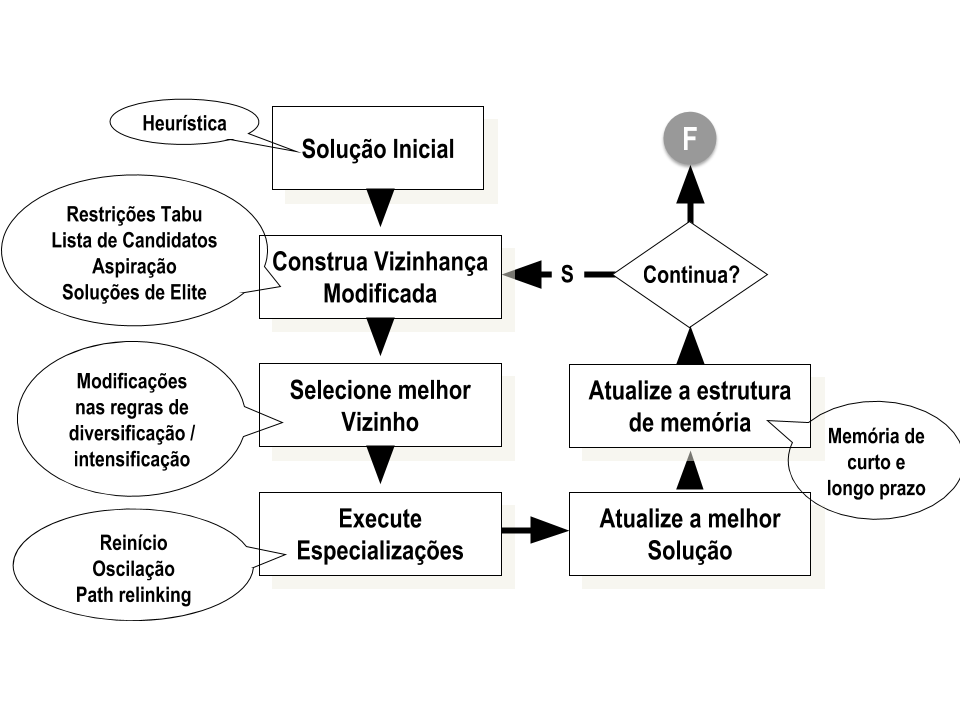
\includegraphics[scale=0.4]{imagens/tabu.png} \par
\bigskip
    Fonte: \cite[p. 97]{goldbarg}
    \label{taboo-image}
\end{figure}

O Algoritmo 1 presente na paǵina \pageref{pseudocodigo-busca-tabu}, representa em pseudocódigo um algoritmo de busca tabu. A variável $p_{max}$ controla o máximo de iterações. A variável $q_{max}$ controla as iterações sem melhoria. \emph{N(s)} simboliza a vizinhança da configuração \emph{s} e \emph{f(s)} representa o valor da configuração \emph{s}.

\makeatletter
\renewcommand{\ALG@name}{Algoritmo}
\makeatother
\renewcommand{\listalgorithmname}{Lista de Algoritmos}

\algrenewcommand\algorithmicend{\textbf{fim}}
\algrenewcommand\algorithmicdo{\textbf{faça}}
\algrenewcommand\algorithmicwhile{\textbf{enquanto}}
\algrenewcommand\algorithmicfor{\textbf{para}}
\algrenewcommand\algorithmicif{\textbf{se}}
\algrenewcommand\algorithmicthen{\textbf{então}}
\algrenewcommand\algorithmicelse{\textbf{senão}}
\algrenewcommand\algorithmicreturn{\textbf{devolve}}
\algrenewcommand\algorithmicfunction{\textbf{função}}
\algrenewtext{EndWhile}{\algorithmicend\ \algorithmicwhile}
\algrenewtext{EndFor}{\algorithmicend\ \algorithmicfor}
\algrenewtext{EndIf}{\algorithmicend\ \algorithmicif}
\algrenewtext{EndFunction}{\algorithmicend\ \algorithmicfunction}
\algnewcommand\algorithmicto{\textbf{até}}
\algrenewtext{For}[3]%
{\algorithmicfor\ #1 $\gets$ #2 \algorithmicto\ #3 \algorithmicdo}
\begin{algorithm}
\caption{Busca tabu \cite[p. 89]{goldbarg}} 
\begin{algorithmic}[1]
\item \textbf{gerar} uma solução inicial \emph{s}, e fazer \emph{s}* := \emph{s}
\item \textbf{inicializar} a Lista Tabu (T)
\item \textbf{inicializar} contadores \emph{p} e \em{q}

\While{$p \neq p_{max}$ e $q \neq q_{max} $}
    \State \textbf{selecionar} o melhor vizinho $s' \in N(s) \setminus T$ 
    \State \textbf{selecionar} o melhor vizinho $s'' \in N(s) \cap T$ 
    \State \If{$f(s'') < f(s') $ e $f(s'') < f(s^*)$}
    \State {$s' \gets s''$}  \Comment{Aspiração} 
    \EndIf
    
    \State \If{$f(s') < f(s^*)$}
    \State {$s^* \gets s'$}
    \State {$q \gets 0$}
    \EndIf
    
    \State \If{$f(s') < f(s)$}
    \State \textbf{colocar} o movimento inverso $(s', s)$ na lista \emph{T}
    \State \textbf{atualizar} \emph{T}
    \EndIf
    
    \State{$s \gets s'$}
    \State{$p \gets p+1$}
    \State{$q \gets q+1$}
\EndWhile
\item \textbf{Devolver} a solução \emph{s}*
\label{pseudocodigo-busca-tabu}
\end{algorithmic}
\end{algorithm}


\subsection*{Colônia de Formigas e Enxame de Abelhas}
Conforme dito anteriormente, muitos métodos meta-heurísticos são inspirados em fenômenos químicos, biológicos, sociais e naturais, como é o caso da Colônia de Formigas e Enxame de Abelhas. Algoritmos em Colônia de Formigas e Enxame de Abelhas são pautados na capacidade de como organismos simples com conceitos modestos de inteligência -- geralmente associados a insetos ou animais de cognição simples -- são capazes de atuar socialmente em conjunto e criar uma organização robusta.

Esta forma de organização social com razoável grau de autonomia é denominado de \emph{Inteligência Coletiva} e um dos precursores do estudo foi William Morton Wheeler, em 1911. Esta forma de inteligência é tão extraordinária que o Prêmio Nobel de 1911, Maurice Maeterlinck, já questionava em seu livro \emph{La Vie des Abeilles} e vários estudos posteriores foram realizados com os mais diversos tipos de insetos \cite{Dorigo2010}. A definição segundo Bonabeau \emph{et al.} \citeyear{bonabeau1999swarm}:

\begin{quote}
Inteligência Coletiva é uma abordagem que permite o desenvolvimento de algoritmos de processamento distribuído inspirados no comportamento de insetos sociais ou de outras sociedades animais.
\end{quote}
\rightline{\cite[p. 7]{bonabeau1999swarm}}

Na área de Otimização Combinatória, os precursores na utilização da Colônia de Formigas foram Beckers \emph{et al.} \citeyear{Beckers1992TrailsAU}, onde foi demonstrado através de um experimento que formigas são capazes de encontrar o caminho mais curto entre o formigueiro e uma fonte de alimentação explorando coletivamente o feromônio que as formigas deixam no chão enquanto caminha; e Colorni \emph{et al.} \citeyear{colorni1992distributed}, que ainda em 1992 publicaram estudo sobre otimização distribuída baseado em Colônias de Formigas.

Sob o ponto de vista sistêmico, estes algoritmos trabalham através de processos de auto-organização. A auto-organização pode ser atribuída a um sistema aberto -- um sistema que permite troca de energia com o ambiente -- que contém a propriedade de conseguir crescer em complexidade de forma organizada sem que exista um guiamento centralizado ou gestão externa ao sistema.

Uma característica de sistemas auto-organizados é que eles emergem padrões. Um padrão é um arranjo privado e organizado de objetos que é preservado no espaço e no tempo. Quando emergentes, estes arranjos permitem que as propriedades do sistema se alterem de forma organizada.

O processo que se opõe à desorganização (\emph{entropia}) é denominado de \emph{negentropia} ou \emph{sintropia}. O Nobel da Física Erwin Schrödinger, distinguiu sistemas com tendências entrópicas e outros que possuem dispositivos negentrópicos e que são capazes de se organizar em níveis cada vez mais complexos e se auto-organizar e regenerar. 

Os algoritmos de Colônia de Formigas são compostos de agentes (\emph{formigas}) que cooperam globalmente para encontrar uma solução. À medida que as soluções são construídas, estruturas de vizinhança ou especiais são marcadas como forma de comunicação. Essa comunicação é empregada assim como a utilização de feromônios na organização das formigas para a construção de uma solução aos passos da formiga que está procurando alimento. Desta forma, a construção da solução percorre uma trilha de decisões marcadas anteriormente.

Algoritmos de Colônia de Formigas seguem algumas características importantes:
\begin{itemize}
    \item As formigas não se comunicam diretamente;
    \item Cada formiga constrói uma solução movendo-se em uma sequência finita de estados.
    \item Estes movimentos são feitos de acordo com probabilidade que leva em consideração informações da própria formiga (memória simples de ações locais) e da trilha de feromônio (ações globais)
\end{itemize}

\chapter*{ANEXO E -- K- Nearest Neighbor}
\label{anexo-k-nearest}
Para realizar o agrupamento de candidatos a serem integrados numa possível rota, a partir do ponto de origem do motorista, é possível utilizar um algoritmo de \emph{ Supervised Machine-Learning }chamado \emph{K-Nearest Neighbour}(KNN). O algoritmo tem o seguinte funcionamento:

A ideia principal do algoritmo é resolver problemas de classificação e regressão. Por ser supervisionado, ele necessita de interação humana no recebimento de entradas e retroalimentação de dados para melhorar seu desempenho. O KNN faz o agrupamento dos dados tendo o princípio inicial de que dados semelhantes têm maior proximidade (funções de distância euclidiana), tendo isso, a classificação ocorre de modo que K é o número de dados a serem avaliados para o agrupamento do KNN. Por ser um algoritmo que requer retroalimentação de dados, é necessário várias execuções para se atingir um valor de K que seja adequado ao problema.

Colocando o KNN no contexto do projeto, é possível realizar a classificação por  proximidade a partir de pontos geográficos do mapa, que no caso, seriam a semelhança entre os usuários. Após a comparação dos dados é definido a distância entre eles, e assim, o KNN vai classificando-os e agrupando-os por regiões de origem e destino semelhantes.
\begin{table}[H]
\centering
\resizebox{\textwidth}{!}{%
\begin{tabular}{cc}
\hline
\textbf{Referência} & \textbf{Tema} \\ \hline
\cite{DIAS2014122} & An Inverted Ant Colony Optimization approach to traffic \\ \hline
\cite{ESCARIO2015390} & Ant Colony Extended: Experiments on the Travelling Salesman Problem \\ \hline
\cite{Marinakis2010} & Honey Bees Mating Optimization algorithm for large scale vehicle routing problems \\ \hline
\cite{MARINAKIS20114684} & Honey bees mating optimization algorithm for the Euclidean traveling salesman problem \\ \hline
\end{tabular}%
}
\caption{Trabalhos relacionados que utilizaram práticas de colônia de formigas.}
\label{colonia-relacionados}
\end{table}